	\clearpage
	\subsubsection{QLearning}
	
\paragraph{}	Q-learning es una t�cninca que funciona aprendiendo una funci�n en base a acciones-valores que devuelve el refuerzo esperado por tomar la acci�n dada en un estado dado y siguiendo una pol�tica fija. Lo importante es que no requiere aprender el modelo del problema.
	
	
\paragraph{}El modelo del problema consiste en un agente, estados S, y un n�mero de acciones por estado A. Realizando las acci�nes , el agente puede moverse de estado a estado. Cada estado provee al agente de una recompenza (un n�mero natural en nuestro caso) o castigo (una recompenza negativa). El objetivo del agente es maximizar la recompenza total. Lo cual logra aprendiendo que acci�n es optima para cada estado.

\paragraph{}El algoritmo, por lo tanto, posee una funci�n que calcula la calidad de un par estado-acci�n.

$Q: S \times A \leftarrow \Re$

\paragraph{}Antes que el aprendizaje empiece, la funci�n Q retorna un valor fijo, elegido por el dise�ador del algoritmo. Luego, cada vez que el agente recibe una recompenza, nuevos valores son calculados para cada combinaci�n de estado-acci�n de S x A. El nucleo del algoritmo es una simple actualzaci�n iterada de valores, la cual actualiza los valores en base a nueva informaci�n.


$$Q(s_t,a_t) \leftarrow \underbrace{Q(s_t,a_t)}_{\footnotesize{\textrm{ viejo valor}}} + \underbrace{\alpha}_{\footnotesize{\textrm{tasa aprendizaje}}}*\left[ \overbrace{ \underbrace{r_{t+1}}_{\footnotesize{\textrm{ recompenza}}} + \underbrace{\gamma}_{\footnotesize{\textrm{factor de descuento}}}* \underbrace{\max_aQ(s_{t+1},a)}_{\footnotesize{\textrm{m�ximo valor futuro}}}}^{\footnotesize{\textrm{recompenza descontada esperada}}} - \underbrace{Q(s_t,a_t)}_{\footnotesize{\textrm{ viejo valor}}}\right]  $$


Un episodio del algoritmo termina cuando el estado $s_{t+1}$ es un estado final.


\paragraph{ Influencia de las varibles en el algoritmo.}

\paragraph{}\textbf{$\alpha$ (Learning rate)}\\
 La tasa de aprendizaje es el que determina que importancia darle a la nueva informaci�n, un factor cerca de 0 implica que el agente aprenda muy poco y una tasa cerca de 1 implica que el agente considerar� mayormente la informaci�n reciente.

\paragraph{}\textbf{$\delta$ (Discount factor)}\\
 El factor de descuento determina la importancia de futuras recompenzas. Un factor cerca de cero har� que el agente concidere solo su acci�n en el momento y no sus consecuencias futuras, contrario al caso de un factor cerca de uno donde el agente conciderara las recompenzas a largo plazo. (si el factor es mayor a uno Qleaning diverge)

\paragraph{Implementaci�n:}

Q learning usa una tabla para almacenar los datos obtenidos, en nuestro caso un simple diccionario con claves (acci�n,estado) y el valor de la funci�n Q como valor. A continuaci�n, veremos el pseudoc�digo utilizado:

	\clearpage
		\begin{figure}[h!]
			\centering
			\includegraphics[width=0.5\textwidth]{qLearning.png}
			\caption{Algoritmo QLearning}
		\end{figure}
	
	
	\subsubsection{Sarsa}

		\begin{figure}[h!]
		\centering
		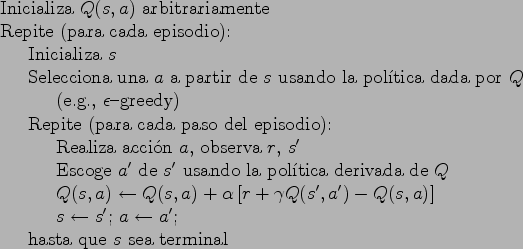
\includegraphics[width=0.5\textwidth]{Sarsa.png}
		\caption{Algoritmo Sarsa}
		\end{figure}
	
	
	\subsubsection{Sarsa ($\lambda$)}	

		\begin{figure}[h!]
			\centering
			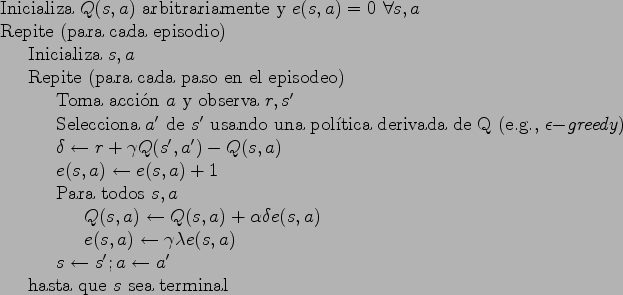
\includegraphics[width=0.5\textwidth]{SarsaLambda.png}
			\caption{Algoritmo Sarsa ($\lambda$)}

		\end{figure}
	
	\subsubsection{Dyna-Q}
		
		\begin{figure}[h!]
			\centering
			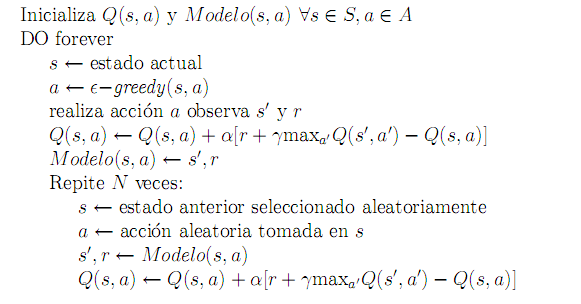
\includegraphics[width=0.5\textwidth]{Dyna.png}
			\caption{Algoritmo Dyna-Q}
		\end{figure}
	
	